\documentclass{standalone}
\usepackage{tikz}
\usepackage{ctex,siunitx}
\setCJKmainfont{Noto Serif CJK SC}
\usepackage{tkz-euclide}
\usepackage{amsmath}
\usetikzlibrary{patterns, calc,3d}
\usetikzlibrary {decorations.pathmorphing,decorations.pathreplacing,decorations.shapes}
\tikzset{label style/.append style={font=\small}}
\begin{document}
\small
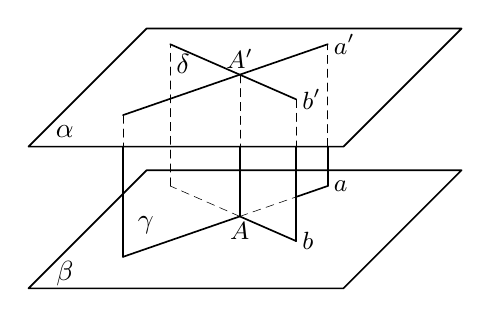
\begin{tikzpicture}[>=latex,scale=1.0,inner sep=2pt]
  \tkzDefPoints{0/0/O',4/0/B',5.5/1.5/C',1.5/1.5/D',0/1.8/O,1.2/0.4/M,3.8/1.3/a,1.8/1.3/P,3.4/0.6/b}
  \tkzInterLL(M,a)(P,b)\tkzGetPoint{A}
  \tkzDefPointsBy[translation=from O' to O](A,B',C',D',M,a,P,b){A',B,C,D,M',a',P',b'}
  \tkzInterLL(A,A')(O,B)\tkzGetPoint{E}
  \tkzInterLL(M,M')(O,B)\tkzGetPoint{F}
  \tkzInterLL(a,a')(O,B)\tkzGetPoint{G}
  \tkzInterLL(P,P')(O,B)\tkzGetPoint{H}
  \tkzInterLL(b,b')(O,B)\tkzGetPoint{I}
  \tkzInterLL(M,a)(b,b')\tkzGetPoint{J}
  \tkzDrawPolygon[semithick](O',B',C',D')
  \tkzDrawPolygon[semithick](O,B,C,D)
  \tkzDrawSegments[semithick](M',a' P',b' M,A b,A A,E M,F b,I a,G J,a)
  \tkzDrawSegments[densely dashed](A',E M',F b',I P,P' G,a' A,J A,P)
  \tkzLabelAngle[pos=0.5](B',O',D'){$\beta$}
  \tkzLabelAngle[pos=0.5](B,O,D){$\alpha$}
  \tkzLabelAngle[pos=0.5](A,M,M'){$\gamma$}
  \tkzLabelAngle[pos=0.3](P,P',A'){$\delta$}
  \tkzLabelPoints(A)
  \tkzLabelPoints[right](a,a',b,b')
  \tkzLabelPoints[above](A')
\end{tikzpicture}
\end{document}